\documentclass{article}%
\usepackage[T1]{fontenc}%
\usepackage[utf8]{inputenc}%
\usepackage{lmodern}%
\usepackage{textcomp}%
\usepackage{lastpage}%
\usepackage[head=40pt,margin=0.5in,bottom=0.6in]{geometry}%
\usepackage{graphicx}%
%
\title{\textbf{Denuncian que el gobierno prepara la expropiación de 71 fincas ganaderas}}%
\author{Eleonora Delgado | eldelgado@el{-}nacional.com | San Cristóbal}%
\date{18/09/2018}%
%
\begin{document}%
\normalsize%
\maketitle%
\textbf{URL: }%
http://www.el{-}nacional.com/noticias/economia/denuncian{-}que{-}gobierno{-}prepara{-}expropiacion{-}fincas{-}ganaderas\_252138\newline%
%
\textbf{Periodico: }%
EN, %
ID: %
252138, %
Seccion: %
Economía\newline%
%
\textbf{Palabras Claves: }%
Sociedad\newline%
%
\textbf{Derecho: }%
3.1%
, Otros Derechos: %
NO\_TIENE%
, Sub Derechos: %
3.1.1%
\newline%
%
\textbf{EP: }%
NO\newline%
\newline%
%
\textbf{\textit{Campesinos y funcionarios encapuchados y armados de la FAES tomaron por la fuerza, el domingo pasado, varias hectáreas del predio La Unión, en el estado Táchira ~}}%
\newline%
\newline%
%
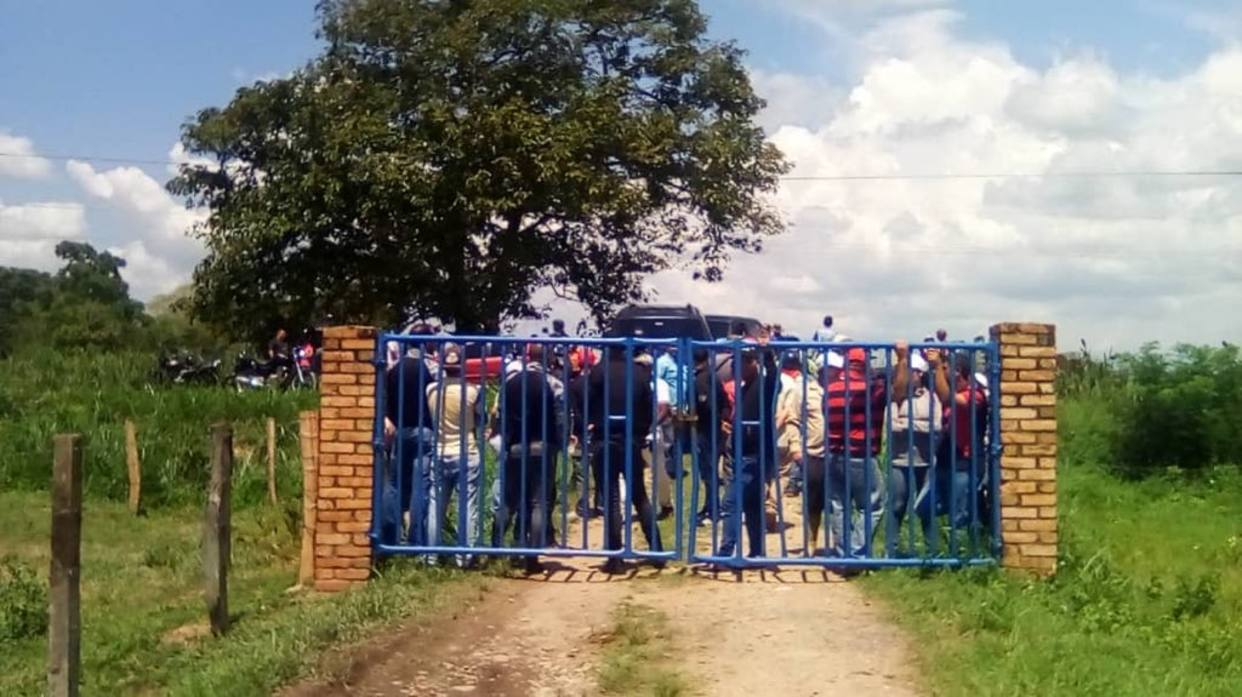
\includegraphics[width=300px]{254.jpg}%
\newline%
%
Carlos Albornoz, presidente del Instituto Venezolano de Carne y Leche, y Armando Chacín, titular de~la Federación Nacional~de Ganaderos de Venezuela, denunciaron que el gobierno prepara la expropiación~de 71 fincas productores de carne y leche.%
\newline%
%
Los directivos se basan en un hecho ocurrido el domingo pasado. Ese día un grupo integrado por aproximadamente 90 personas, acompañado de funcionarios encapuchados y armados de~la Fuerza~de Acciones Especiales de~la Policía Nacional~Bolivariana, llegó a la finca~La Unión, en el kilómetro 93 en la vía Orope{-}La Fría, del municipio García de Hevia, noroeste del Táchira, en la frontera con Colombia. La intención fue invadir la parte trasera del predio, que en total tiene una extensión de~183 hectáreas.%
\newline%
%
“Tenemos información de que el gobierno le hará lo mismo a más de 71 fincas en Táchira. No entendemos por qué en un país donde la gente deambula buscando comida, todavía el gobierno insiste en expropiar y eliminar unidades que aún son útiles al producir carne y leche”, dijo Chacín.%
\newline%
%
Aseguró que si la intención del Ejecutivo es expropiar las fincas para colocar en el mercado a precio regulado la carne y la leche que producen, la medida duraría poco. “Ojalá que el gobierno tenga éxito en la puesta en marcha de las medidas económicas, pero dificulto que un sector económico pueda sobrevivir a pérdida. Una vez que nos comamos toda la carne y el productor agropecuario no tenga capacidad para sostenerse, vamos a tener que ir a tocar la puerta de los vecinos para no morir de hambre y tener algo de alimento para la población. No hay posibilidad alguna de que este país pueda alimentar a 30 millones de personas si se acaba con el campo venezolano. Cada día tenemos menos qué comer”, afirmó.%
\newline%
%
Albornoz añadió que expropiar 71 predios es “una cifra muy dura, muy contundente”. “Nuestro llamado es a los productores, a que sigan unidos y resistiendo”.%
\newline%
%
El ganadero también responsabilizó a autoridades municipales de participar en la acción contra la finca~La Unión.~“El alcalde de García Hevia, Willington Vivas, ~haciendo uso excesivo~~de sus atribuciones reunió gente de caseríos aledaños, ofreciéndoles dinero, para que se anotaran en una lista para que el INTI les hiciera una adjudicación por un lote de tierra en la parte trasera de la finca, que está apenas a cinco kilómetros de la zona donde operan peligrosísimos grupos irregulares en la frontera con Colombia”.%
\newline%
%
Albornoz contó que a los dueños de la finca les robaron 430 reses el año pasado y las autoridades hicieron caso omiso de la denuncia. “Esa finca familiar lleva más de 60 años operando y a pesar del robo produce 270.000 kilos de carne al año y más de~1.020.000 litros~de leche”, indicó Chacín.%
\newline%
%
El presidente de Fedenaga señaló que~La Unión~está ubicada en un área de permanente disputa entre grupos que se dedican al contrabando, incluso funcionarios policiales y de~la Alcaldía~de García de Hevia.%
\newline%
%
Laidy Gómez, gobernadora del Táchira, declaró que la intención de tomar el lugar a la fuerza es para avalar actividades ilícitas que estarían ligadas al contrabando. “No vamos a permitir que en el estado Táchira se vulnere el derecho a la propiedad.~~No seremos cómplices de dictámenes administrativos sobre propiedades que están a~300 metros~de la frontera, donde se puede generar el ilícito del contrabando”, advirtió Gómez.%
\newline%
%
La cifra%
\newline%
%
270.000 kilos de carne al año y más de~1.020.000 litros~de leche produce la finca~La Unión, ubicada en el estado Táchira, pese a que en 2017 le robaron 430 reses%
\newline%
%
\end{document}